\documentclass[a4paper, 12pt, final, garamond]{book}
\usepackage{cours-preambule}

\raggedbottom

\makeatletter
\renewcommand{\@chapapp}{Optique -- chapitre}
\makeatother

\begin{document}
\setcounter{chapter}{3}

\chapter{Correction du TD}

\section{Vergence de lentilles accolées}
\begin{enumerate}
    \item Dans cette situation, on a le système $A \opto{\Lc_1}{O_1} A_1
        \opto{\Lc_2}{O_2} A'$, avec $O_1 = O_2 = O$. Une lentille équivalente à
        ce système ferait passer directement de $A$ à $A'$ et aurait une
        distance focale $\obar{OF'}$ telle que
        \begin{equation}\label{eq:vaccol}
            \frac{1}{\OF} = \frac{1}{\OAp} - \frac{1}{\OA}
        \end{equation}
        Pour faire apparaître les vergences des lentilles une et deux, on peut~:
        \begin{enumerate}
            \item Écrire les relations de conjugaison pour les deux lentilles~:
                \begin{equation*}
                    \boxed{\frac{1}{\obar{OF'_1}} = \frac{1}{\obar{OA_1}} -
                    \frac{1}{\obar{OA}}}
                    \quad\text{et}\quad
                    \boxed{\frac{1}{\obar{OF'_2}} = \frac{1}{\obar{OA'}} -
                    \frac{1}{\obar{OA_1}}}
                \end{equation*}

            \item Ou directement dans~\ref{eq:vaccol} ajouter et retirer
                $\frac{1}{\obar{OA_1}}$ dans le terme de droite.
        \end{enumerate}
        Quoiqu'il en soit, on trouve rapidement
        \begin{align*}
            \frac{1}{\OF}     & = \frac{1}{\obar{OF'_1}} + \frac{1}{\obar{OF'_2}}\\
            \Leftrightarrow V & = V_1 + V_2
        \end{align*}
    \item Le grandissement de l'ensemble est $\gamma =
        \dfrac{\obar{OA'}}{\obar{OA}}$. Or, $\gamma_1 =
        \dfrac{\obar{OA_1}}{\obar{OA}}$ et
        $\gamma_2 = \dfrac{\obar{OA'}}{\obar{OA_1}}$~; on a donc
        \begin{empheq}[box=\fbox]{equation*}
            \gamma = \gamma_1\gamma_2
        \end{empheq}
\end{enumerate}
\begin{rema}[label=rema:prod_gamma, hand]{produit des grandissements}
    Si le théorème des vergences (c'est son nom) ne vaut que pour des lentilles
    accolées (une version plus générique s'écrit $V = V_1 + V_2 -
    \obar{O_1O_2}V_1V_2$), l'expression du grandissement \textbf{vaut pour toute
    association}.
\end{rema}

\section{L'œil hypermétrope et sa correction}
\begin{center}
    \begin{NCdefi}[width=.9\linewidth, sidebyside]{Données}
        \begin{itemize}
            \item Œil = lentille $(\Lc, S)$ ;
            \item $\obar{SE} = \SI{17}{mm}$ ;
            \item $\obar{SA} = -\infty \Rightarrow \obar{SA'} = \obar{SE} +
                \SI{1.5}{mm}$
        \end{itemize}
        \tcblower
        \tcbsubtitle[before skip=\baselineskip,
        colback = green!50!black,
        colframe = green!50!black]{Schéma}
        \begin{center}
            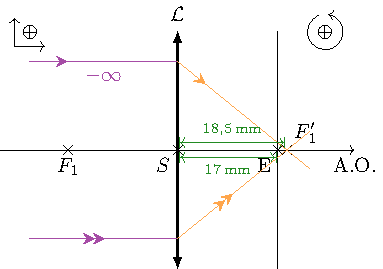
\includegraphics{oeil_hyper-data.pdf}
        \end{center}
    \end{NCdefi}
\end{center}

\begin{enumerate}
    \item ~
        \begin{tcbraster}[raster columns=5, raster equal height=rows]
            \begin{NCprop}{Résultat attendu}
                \[\obar{SF'}\]
            \end{NCprop}
            \begin{NCrapp}[raster multicolumn=2]{Outil}
                On trouve le point focal image d'un système en étudiant l'image d'un
                objet à l'infini.
            \end{NCrapp}
            \begin{NCexem}[raster multicolumn=2]{Application}
                Ici, la lecture de l'énoncé donne directement la réponse~: le point
                focal image et \SI{1.5}{mm} derrière la rétine. On a donc \[\obar{SF'} =
                \SI{18.5}{mm}\]
            \end{NCexem}
        \end{tcbraster}
    \item L'œil n'est pas assez convergent, il faudrait que les rayons se
        croisent plus tôt sur l'axe optique pour que l'image se forme sur la
        rétine. Il faut donc corriger avec des lentilles correctrices
        convergentes.

    \item ~
        \begin{center}
            \begin{NCdefi}[width=.9\linewidth, sidebyside]{Données}
                \begin{itemize}
                    \item Verre lunette = $(\Lc_v, O)$ ;
                    \item $\obar{OS} = \SI{12}{mm}$ ;
                    \item $\ABb \opto{\Lc_v}{O} \ABa \opto{\Lc}{S} \ABp$
                \end{itemize}
                \tcblower
                \tcbsubtitle[before skip=\baselineskip,
                colback = green!50!black,
                colframe = green!50!black]{Schéma}
                \begin{center}
                    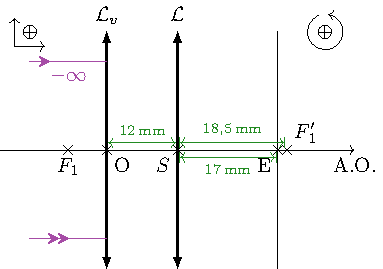
\includegraphics{oeil_hyper-verre.pdf}
                \end{center}
            \end{NCdefi}
        \end{center}
        \begin{enumerate}
            \item ~
                \begin{center}
                    \begin{NCdemo}[width=.5\linewidth]{Rappel}
                        L'image doit se former sur l'écran de la lentille,
                        autrement dit la rétine~: avec $\ABb = -\infty$ on doit
                        avoir $A' = E$.
                    \end{NCdemo}
                \end{center}
            \item ~
                \begin{tcbraster}[raster columns=7, raster equal height=rows]
                    \begin{NCprop}[raster multicolumn=2]{Résultat attendu}

                        Utiliser le fonctionnement physique du système pour
                        déterminer comment associer la lunette à l'œil.

                    \end{NCprop}
                    \begin{NCror}[raster multicolumn=2]{Important !}

                        Attention, \textbf{seul} le remotum de l'œil emmétrope
                        est à l'infini. Vérifiez bien vos définitions.

                    \end{NCror}
                    \begin{NCexem}[raster multicolumn=3]{Application}
                        \begin{center}
                            \begin{tikzpicture}[]
                                \node[] (AB) at (0,0) {$\ABb$};
                                \node[] (A_1B_1) at (2,0) {$\ABa$};
                                \node[] (A'B') at (4,0) {$\ABp$};
                                \draw[->] (AB) -- (A_1B_1)
                                    node [midway, above] {$\Lc_v$}
                                    node [midway, below] {O};
                                \draw[->] (A_1B_1) -- (A'B')
                                    node [midway, above] {$\Lc$}
                                    node [midway, below] {S};
                                \node[below=0.3, Purple!70]
                                    (ABb) at (AB) {$-\infty$};
                                \node[below=0.3, brandeisblue]
                                    (A1B1b) at (A_1B_1) {$A_1 = F'_v$};
                                \node[below=0.3, ForestGreen]
                                    (A1B1bb) at (A1B1b) {$A_1 = R$};
                                \node[below=0.3, orange!70]
                                    (A'B'b) at (A'B') {$A' = E$};
                                \draw[->, Purple!70]
                                    (ABb) to[bend right] (A1B1b.west);
                                \draw[->, orange!70]
                                    (A'B'b) to[bend left] (A1B1bb.east);
                            \end{tikzpicture}
                        \end{center}
                        On a donc $A_1 = F'_v = R$.
                    \end{NCexem}
                \end{tcbraster}
            \item ~
                \begin{tcbraster}[raster columns=2, raster equal height=rows]
                    \begin{NCprop}{Résultats attendus}

                        On cherche $\obar{OF'_v}$ sachant que $F'_v = R$~:
                        l'idée est donc de trouver $R$ de l'œil connaissant sa
                        distance focale et la distance œil-écran

                    \end{NCprop}
                    \begin{NCrapp}{Outil}

                        On va donc utiliser la formule de conjugaison d'une
                        lentille mince~:

                        \[ \frac{1}{\OF} = \frac{1}{\OAp} - \frac{1}{\OA}\]
                    \end{NCrapp}
                \end{tcbraster}
                \begin{center}
                    \begin{NCexem}[width=.9\linewidth]{Application}
                        Avec les données de l'exercice, on a

                        \[\frac{1}{\obar{SF'}} = \frac{1}{\obar{SE}} -
                        \frac{1}{\obar{SR}}\]
                        Soit
                        \begin{equation*}
                           \boxed{\obar{SR} = \frac{\obar{SE}\obar{SF'}}
                           {\obar{SF'}-\obar{SE}}}
                           \quad \text{avec}\quad
                           \left\{
                               \begin{array}{rcl}
                                   \obar{SE} & = & \SI{17}{mm}\\
                                   \obar{SF'} & = & \SI{18.5}{mm}
                                \end{array}
                            \right.
                        \end{equation*}
                        Et \[\boxed{\obar{SR} = \SI{21}{cm}}\]

                        Avec la composition des distances et comme $F'_v = R$,
                        on a finalement

                        \[\boxed{\obar{OF'_v} =
                        \obar{OS} + \obar{SR} = \num{1.2}+\num{20.9} = \SI{22}{cm}}\]
                        Soit \fbox{$V_{\rm verre} = \SI{+4.5}{\de}$}
                    \end{NCexem}
                \end{center}
            \item On a donc 
                \begin{center}
                    \hspace*{-2cm}
                    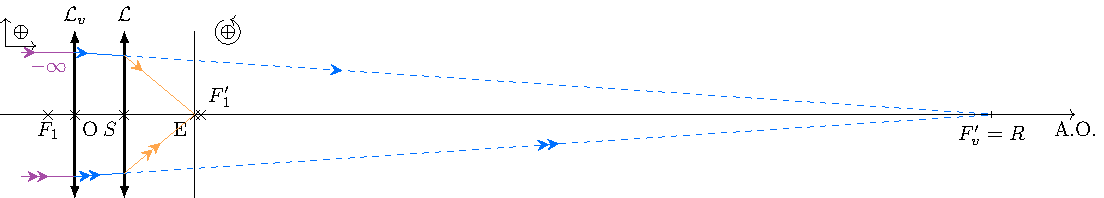
\includegraphics{oeil_hyper-fin}
                \end{center}
        \end{enumerate}
\end{enumerate}

\section{Élargissement d'un faisceau laser}

\begin{minipage}{0.65\linewidth}
    On peut associer deux lentilles, la première divergente de très courte
    focale $f'_1$ ($< 0$) et la seconde convergente de grande focale $f'_2$, à
    condition de faire coïncider le foyer image $F'_1$ de la première avec le
    foyer objet $F_2$ de la seconde. Si $D$ est le diamètre du faisceau final et
    $d$ celui du faisceau initial, alors en utilisant le théorème de Thalès
    $D/f'_2 = -d/f'_1$~; pour $d = \SI{2}{mm}$ et $D = \SI{3}{cm}$, il nous faut
    \begin{empheq}[box=\fbox]{equation*} f'_2 = -15 f'_1
    \end{empheq}
\end{minipage}
\hfill
\begin{minipage}{0.30\linewidth}
    \begin{center}
        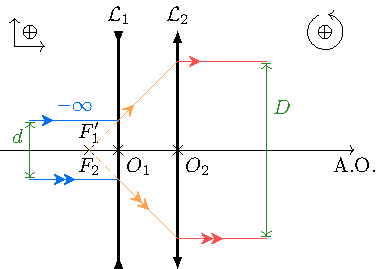
\includegraphics[width=\linewidth]{laser_elarg.pdf}
    \end{center}
\end{minipage}

\section{Étude d'un photocopieur}
\begin{enumerate}
    \item La lentille divergente ne peut pas donner une image réelle si l'objet
        est réel (vérifiez avec la relation de conjugaison). Par conséquent,
        l'image à travers $\Lc_1$ \textbf{ne peut pas être sur le récepteur},
        car cette dernière est virtuelle.

    \item Si $\Lc'$ est divergente, l'image de $A$ est virtuelle, comme vu
        précédemment~; mais ça sera donc un objet réel pour $\Lc_1$, et on a
        encore le même raisonnement. Ainsi, si une lentille peut fonctionner
        dans ce système, elle ne peut être divergente.

    \item L'image finale est telle que $\obar{O_1A'} = \SI{180}{mm}$, l'objet
        initial est tel que $\obar{O'A} = \SI{-180}{mm}$ et on a $\obar{O'O_1} =
        \SI{24}{mm}$. Avec le système $A \opto{\Lc'}{O'} A_1
        \opto{\Lc_1}{O_1} A'$, on sait qu'on a les relations
        \begin{equation*}
            \left\{
                \begin{aligned}
                    \frac{1}{f'} & = \frac{1}{\obar{O'A_1}} -
                        \frac{1}{\obar{O'A}}\\
                    \frac{1}{f'_1} & = \frac{1}{\obar{O_1A'}} -
                    \frac{1}{\obar{O_1A_1}}
                \end{aligned}
            \right.
            \Leftrightarrow
            \left\{
                \begin{aligned}
                        f' & = \left( \frac{1}{\obar{O'A_1}} -
                        \frac{1}{\obar{O'A}} \right)^{-1}\\
                    \obar{O_1A_1} & = \left( \frac{1}{\obar{O_1A'}} -
                                             \frac{1}{f'_1} \right)^{-1}
                \end{aligned}
            \right.
            \Leftrightarrow
            \left\{
                \begin{aligned}
                    f' & =
                    \frac{\obar{O'A_1}\times\obar{O'A}}{\obar{O'A}-\obar{O'A_1}}\\
                    \obar{O_1A_1} & = \frac{f'_1\times\obar{O_1A'}}{f'_1-\obar{O_1A'}}
                \end{aligned}
            \right.
        \end{equation*}
        On en déduit $\DS\obar{O'A_1} = \obar{O_1A_1} - \obar{O_1O'} =
        \frac{f'_1\times\obar{O_1A'}}{f'_1-\obar{O_1A'}} - \obar{O_1O'}$~; avec
        $ \left\{
            \begin{array}{rcl}
                f'_1 & = & \SI{-90}{mm}\\
                \obar{O_1A'} & = & \SI{180}{mm}\\
                \obar{O_1O'} & = & \SI{-24}{mm}
            \end{array}
        \right.$ on a
        \begin{empheq}[box=\fbox]{equation*}
            \obar{O'A_1} = \SI{84}{mm}
        \end{empheq}
        et finalement avec $\obar{O'A} = \SI{-180}{mm}$, on a également
        \begin{empheq}[box=\fbox]{equation*}
            f' = \SI{57}{mm}
        \end{empheq}
    \item $\gamma_{\rm imprim} = \gamma_{\Lc'}\gamma_{\Lc_1}$ en tant
        qu'association de lentilles~; or $\gamma_{\Lc'} =
        \dfrac{\obar{O'A_1}}{\obar{O'A}} = \num{-0.5}$, et $\gamma_{\Lc_1} =
        \dfrac{\obar{O_1A'}}{\obar{O_1A_1}} = 3$~: on a
        \begin{empheq}[box=\fbox]{equation*}
            \gamma_{\rm imprim} = \num{-1.5}
        \end{empheq}
        $|\gamma_{\rm imprim}| > 1$ d'une part, mais pour savoir si on peut
        imprimer en A3 il faut savoir si la \textit{surface} est multipliée par
        2~; $\gamma$ est un grandissement linéique (sur une longueur). Pour la
        surface, on calcule $\gamma_{\rm imprim}^2 = 2.25 > 2$~: on peut donc
        transformer du A4 en A3.
\end{enumerate}

\section{Le microscope}

\begin{enumerate}
    \item L'œil visant sans fatigue à l'infini, il faut que l'image par $\Lc_2$
        soit à l'infini. Pour ça, l'image intermédiaire $A_1$ de $A$ par $\Lc_1$
        doit se situer dans le plan focal objet de $\Lc_2$. Autrement dit, on
        doit avoir $\obar{F'_1A_1} = \obar{F'_1F_2}$. Ceci ce traduit par la
        schématisation optique $AB \opto{\Lc_1}{O_1} \underbrace{A_1B_1}_{A_1 =
        F_2}\opto{\Lc_2}{O_2}
        +\infty$. On utilise donc la relation de conjugaison pour la lentille
        $\Lc_1$ avec origine au foyer~:
        \begin{equation*}
            \obar{FA}\obar{F'A'} = -f'{}^2
        \end{equation*}
        et avec les notations choisies, $\obar{F_1A}\obar{F'_1A_1} = -f'_1{}^2$.
        On en tire directement
        \[\boxed{\obar{F_1A} = \frac{-f'_1{}^2}{\Delta}}
            \quad\text{avec}\quad
            \left\{
                \begin{array}{rcl}
                    f'_1 & = & \SI{5}{mm}\\
                    \Delta & = & \SI{250}{mm}
                \end{array}
            \right.
            \quad\text{soit}\quad
        \boxed{\obar{F_1A} = \SI{-0.1}{mm}}\]
    \item ~
        \begin{center}
            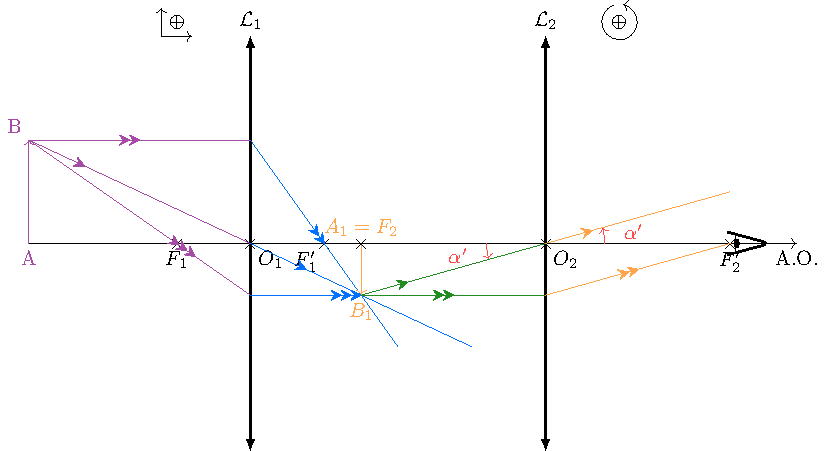
\includegraphics[width=\linewidth]{microscope.pdf}
            \label{fig:microscope}
        \end{center}

    \item Avec le schéma ci-dessus et dans l'hypothèse des conditions de Gauss
        ($\tan\theta \approx \theta$), $\alpha' = \dfrac{\obar{A_1B_1}}{-f'_2}$.
        On veut relier $\obar{A_1B_1}$ à $\ABb$ puisqu'on aura $\alpha =
        \dfrac{\ABb}{-\Delta}$~: on utilise pour ça l'expression du grandissement
        avec origine aux foyers (on connaît $\obar{F_1A}$)~:
        \begin{gather*}
            \gamma = \frac{\ABa}{\ABb} = - \frac{\obar{O_1F_1}}{\obar{F_1A}}\\
            \Leftrightarrow \ABa = \ABb \frac{f'_1}{\obar{F_1A}}
        \end{gather*}
        Ainsi, $\DS G = \frac{\alpha'}{\alpha} = \frac{- \frac{f'_1}{f'_2}
        \frac{\ABb}{\obar{F_1A}}}{ \frac{\ABb}{-\Delta}}$ donc
        \[\boxed{G = -\frac{\Delta^2}{f'_1f'_2}}
        \quad\text{avec}\quad
        \left\{
            \begin{array}{rcl}
                \Delta & = & \SI{25}{cm}\\
                f'_1 & = & \SI{5}{mm}\\
                f'_2 & = & \SI{25}{mm}
            \end{array}
        \right.\quad\text{soit}\quad
        \boxed{G=-500}\]

\end{enumerate}

\section{Lunettes astronomiques de Kepler et Galilée}
\subsection{Kepler}

\begin{center}
    \begin{NCdefi}[width=.8\linewidth]{Données}
    Association de deux lentilles~:
    \begin{enumerate}
        \item $\Lc_1$ « objectif », vergence $V_1 = \SI{3.125}{\de}$, diamètre $D
            = \SI{30}{mm}$ ;
        \item $\Lc_2$ « oculaire », vergence $V_2 = \SI{25}{\de}$.
    \end{enumerate}
\end{NCdefi}
\end{center}

\subsubsection{}

\begin{tcbraster}[raster columns=7, raster equal height=rows]
    \begin{NCprop}[raster multicolumn=2]{Résultat attendu}
        Focales de lentilles
    \end{NCprop}
    \begin{NCrapp}[raster multicolumn=2]{Outil du cours}
        $$V = \dfrac{1}{f'}$$
    \end{NCrapp}
    \begin{NCexem}[raster multicolumn=3, valign=top]{Application}
        \[ \boxed{\obar{O_1F'_1} = \SI{32}{cm}} \quad\text{et}\quad
        \boxed{\obar{O_2F'_2} = \SI{4}{cm}} \]
    \end{NCexem}
\end{tcbraster}

\subsubsection{}
\begin{tcbraster}[raster columns=2, raster equal height=rows]
    \begin{defi}{Système afocal}
        Est afocal un système pour lequel un objet initial à l'infini donne une
        image finale à l'infini.
    \end{defi}
    \begin{inte}{Intérêt d'un système afocal}
        Un système afocal présente comme intérêt de permettre à un œil emmétrope
        d'observer sans fatigue, étant donné que l'image sortant du système est à
        l'infini (voir cours).
    \end{inte}
\end{tcbraster}

\subsubsection{}\label{sssec:k_encomb}

\begin{tcbraster}[raster columns=7, raster equal height=rows]
    \begin{tcolorbox}[blankest, raster multicolumn=3, space to=\myspac]
        \begin{tcbraster}[raster columns=1]
            \begin{NCprop}[]{Résultat attendu}
                $$\obar{O_1O_2}$$
            \end{NCprop}
            \begin{NCrapp}[add to natural height=\myspac]{Outils du cours}
                Règles de construction de rayons~:
                \begin{enumerate}
                    \item Un rayon provenant de l'infini émerge d'une lentille en croisant
                        l'axe optique au plan focal image ;
                    \item Des rayons se croisant dans le plan focal objet d'une lentille
                        émergent parallèles entre eux.
                \end{enumerate}
                Relation de Chasles~:
                \[ \obar{O_1O_2} = \obar{O_1F_1'} + \obar{F_1'O_2} \]
            \end{NCrapp}
        \end{tcbraster}
    \end{tcolorbox}
    \begin{NCexem}[raster multicolumn=4]{Application}
        Pour que tous les rayons sortant de la lunette soient parallèles entre eux
        (donnant donc une image à l'infini), il faut que tous les rayons à
        l'intérieur passent par le plan focal objet de son oculaire.\bigbreak
        Or, tous les rayons arrivent dans la lunette parallèles entre eux (objet
        initial à l'infini) ; il se croisent donc dans le plan focal image de
        l'objectif. \bigbreak
        Pour que la condition soit vérifiée, il faut donc simplement que les plans
        focaux image de $\Lc_1$ et objet de $\Lc_2$ soient confondus ; autrement dit~:
        \[ \boxed{F_1' = F_2} \]
        On a alors $\obar{O_1O_2} = \obar{O_1F_1'} + \obar{F_2O_2}$, et finalement
        \[ \boxed{\obar{O_1O_2} = \SI{+36}{cm}} \]
    \end{NCexem}
\end{tcbraster}

\subsubsection{}
Pour cette question, le placement de l'image intermédiaire ne nécessite que le
tracé du rayon passant par $O_1$, étant donné que son intersection avec le plan
focal image donnera la position de $B_1$~:

\begin{center}
    \begin{NCdemo}[width=\linewidth]{Rappel}
        \begin{itemize}
            \item Deux rayons parallèles avant le système optique se coupent
                dans le plan focal image ;
            \item Deux rayons qui se coupent dans le plan focal objet émergent
                parallèles entre eux.
        \end{itemize}
    \end{NCdemo}
\end{center}

On peut donc facilement tracer les rayons émergents du «~pinceau~» (i.e.\
l'espace entre les deux rayons entrant) puisqu'ils doivent se croiser en $B_1$.
Sur le schéma suivant, les rayons sortant sont également tracés, et cette fois
on utilise la seconde partie du rappel précédent~: les deux rayons bleus se
coupant en $B_1$ émergent parallèle entre eux, et il suffit de construire un
rayon émergent de $B_1$ (par exemple celui passant par $O_2$ et qui n'est pas
dévié) pour trouver l'angle de sortie.

\begin{center}
    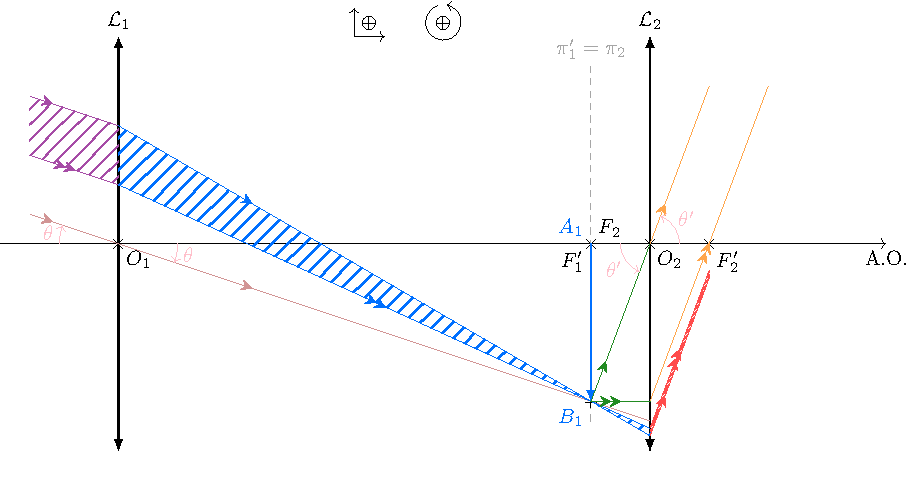
\includegraphics{kepler.pdf}
\end{center}

\subsubsection{}
\begin{tcbraster}[raster columns=6, raster equal height=rows]
    \begin{tcolorbox}[blankest, raster multicolumn=1, space to=\myspace]
        \begin{tcbraster}[raster columns=1]
            \begin{NCprop}[add to natural height=\myspace, valign=top]
                {Résultat attendu}
                $$G$$
            \end{NCprop}
            \begin{NCrapp}{Outil}
                \[ G = \frac{\theta'}{\theta}\]
            \end{NCrapp}
        \end{tcbraster}
    \end{tcolorbox}
    \begin{NCexem}[raster multicolumn=2]{Application}
        Avec le tracé sur le schéma et en considérant des petits angles,
        $\DS \theta' = \frac{\ABa}{\obar{O_2F_2}} > 0$ et $\DS \theta =
        \frac{\ABa}{\obar{O_1F_1'}} < 0$, soit \[ G = \frac{f_1'}{-f_2'} = -8\]
    \end{NCexem}
    \begin{NCror}[raster multicolumn=3]{Attention}
        Pour bien voir si un angle est positif ou négatif, il faut se donner un
        sens dans lequel compter positivement, tracer les angles depuis l'axe
        optique jusqu'au rayon pour voir le changement de direction et dans la
        formule trigonométrique utiliser les grandeurs dans le bon sens.
    \end{NCror}
\end{tcbraster}

\subsubsection{}\label{sssec:k_cercleo}
\begin{tcbraster}[raster columns=2, raster equal height=rows]
    \begin{defi}{Cercle oculaire}
        On appelle cercle oculaire l'image de la monture de l'objectif donnée par
        l'oculaire.
    \end{defi}
    \begin{inte}{Utilité du cercle oculaire}
        Il correspond à la section la plus étroite du faisceau sortant de
        l'oculaire, où l'œil reçoit le maximum de lumière.  
    \end{inte}
\end{tcbraster}

\subsubsection{}

\begin{tcbraster}[raster columns=6, raster equal height=rows]
    \begin{tcolorbox}[blankest, raster multicolumn=3, space to=\myspacee]
        \begin{tcbraster}[raster columns=1]
            \begin{NCprop}[raster multicolumn=1,
                add to natural height=\myspacee]{Résultat attendu}
                $$\obar{O_2C_K'}$$
            \end{NCprop}
            \begin{NCrapp}[raster multicolumn=2]{Outil du cours}
                Par définition, $C_K'$ est l'image de $O_1$ par $\Lc_2$. On va
                donc se servir de la relation de conjugaison d'une lentille
                mince~:
                \[ \frac{1}{\OF} = \frac{1}{\OAp} - \frac{1}{\OA} \]
            \end{NCrapp}
        \end{tcbraster}
    \end{tcolorbox}
    \begin{NCexem}[raster multicolumn=3]{Application}
        On a ici $O \equiv O_2$, $F' \equiv F_2'$, $A \equiv O_1$ et $A' \equiv
        C_K'$. On a donc~:
        \[ \frac{1}{\obar{O_2F_2'}} = \frac{1}{\obar{O_2C_K'}} -
        \frac{1}{\obar{O_2O_1}} \]
        et après calculs~:
        \[ \boxed{\obar{O_2C_K'} = \left[ \frac{1}{\obar{O_2O_1}} +
        \frac{1}{\obar{O_2F_2'}}\right]^{-1} = \SI{+4.5}{cm}} \]
    \end{NCexem}
\end{tcbraster}

\subsubsection{}\label{sssec:k_diam}
\begin{tcbraster}[raster columns=6, raster equal height=rows]
    \begin{tcolorbox}[blankest, raster multicolumn=3]
        \begin{tcbraster}[raster columns=1]
            \begin{NCprop}[raster multicolumn=1]{Résultat attendu}
                $$D_K'$$
            \end{NCprop}
            \begin{NCrapp}[raster multicolumn=2]{Outil du cours}
                Le diamètre du cercle oculaire s'apparente à la taille d'un
                objet. On peut donc utiliser le grandissement~:
                \[ \g = \frac{\ABp}{\ABb} = \frac{\OAp}{\OA} \]
            \end{NCrapp}
        \end{tcbraster}
    \end{tcolorbox}
    \begin{NCexem}[raster multicolumn=3]{Application}
        Avec les données de l'énoncé, on obtient~:
        \[ \g = \frac{D_K'}{D} = \frac{\obar{O_2C_K'}}{\obar{O_2O_1}}\]
        et finalement
        \[ \boxed{D_K' = D\times \frac{\obar{O_2C_K'}}{\obar{O_2O_1}} =
        \SI{3.75}{mm}} \]
    \end{NCexem}
    
\end{tcbraster}

\subsection{Galilée}

\subsubsection{}
Si l'oculaire est divergent, cela signifie que $C_3 < 0$. On a donc $C_3 = -
C_2$, d'où le résultat demandé.

\subsubsection{}
On reprend la question \ref{sssec:k_encomb}, avec cette fois des indices « 3 »
au lieu des indices « 2 », et on obtient~:

\begin{tcbraster}[raster columns=2, raster equal height=rows]
    \begin{NCexem}{Application}

        $\obar{O_1O_3} = \obar{O_1F_1'} + \obar{F_3O_3}$ avec $\obar{F_3O_3} =
        \obar{O_3F_3'} = \SI{-4}{cm}$, d'où $\boxed{\obar{O_1O_3} =
        \SI{+28}{cm}}$

    \end{NCexem}
    \begin{inte}{Intérêt}
        La lunette de Galilée est donc plus compacte que la lunette de Kepler !
    \end{inte}
\end{tcbraster}
\vfill
\subsubsection{}

\begin{center}
    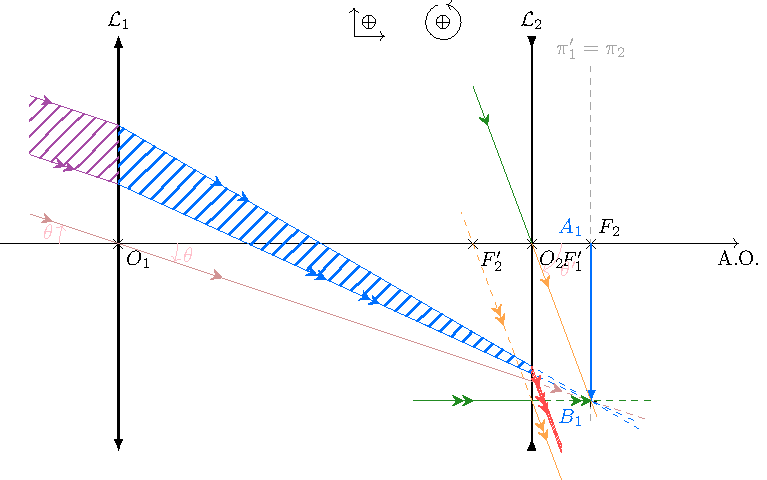
\includegraphics{galilee.pdf}
\end{center}

\subsubsection{}
On reprend la question \ref{sssec:k_cercleo}, avec des indices « 3 » au lieu de
« 2 », et on obtient~:
\begin{tcbraster}[raster columns=3, raster equal height=rows]
    \begin{NCexem}[raster multicolumn=1]{Application}
        \[ \boxed{\obar{O_3C_G'} = \SI{-3.5}{cm}}\]
    \end{NCexem}
    \begin{NCrema}[raster multicolumn=2]{Comparaison}
        On a cette fois un cercle oculaire virtuel. Il faudra placer son œil le plus
        près possible de l'oculaire pour espérer avoir le plus de lumière possible.
    \end{NCrema}
\end{tcbraster}

\subsubsection{}
On reprend la question \ref{sssec:k_diam}~:
\begin{center}
    \begin{NCexem}[width=.3\linewidth]{Application}
        \[ \boxed{D_G' = \SI{3.75}{mm}} \]
    \end{NCexem}
\end{center}

\subsubsection{Comparaison}
\begin{center}
    \begin{tabularx}{.7\linewidth}{|Y*{2}{|Y}|}\hline
        \rowcolor{gray!15} & Avantages & Inconvénients \\\hline
        \cellcolor{gray!15} Lunette Galilée & + compacte\smallbreak image droite &
        cercle oculaire virtuel \\\hline
        \cellcolor{gray!15} Lunette Kepler & Grande clarté \smallbreak Cercle
        oculaire réel & - compacte \smallbreak image renversée \\\hline
    \end{tabularx}
\end{center}


\end{document}
